\section{SIM TIPS Simulator}

TIPS (Tips Is a Pixel Simulator) is mainly written in Python, but its core is based on aXeSIM, which is written in C and then wrapped in python by TIPS itself. The TIPS official gitlab repository can be found at the link

\url{https://gitlab.euclid-sgs.uk/PF-SIM/SIM_TIPS_Simulator}

Essentially TIPS has three main programs:

\begin{itemize}
\item \verb+EuclidNisSplit.py+: it creates the TIPS fits configuration and catalog files;
\item \verb+EuclidNisDetector.py+: it does the pixel simulation at the single detector level, taking the configuration and catalog files as inputs;
\item \verb+EuclidNisCOmbine.py+: it takes all the 16 detector simulated frames and combines them into a single fits file.
\end{itemize}

\begin{figure}
    \centering
    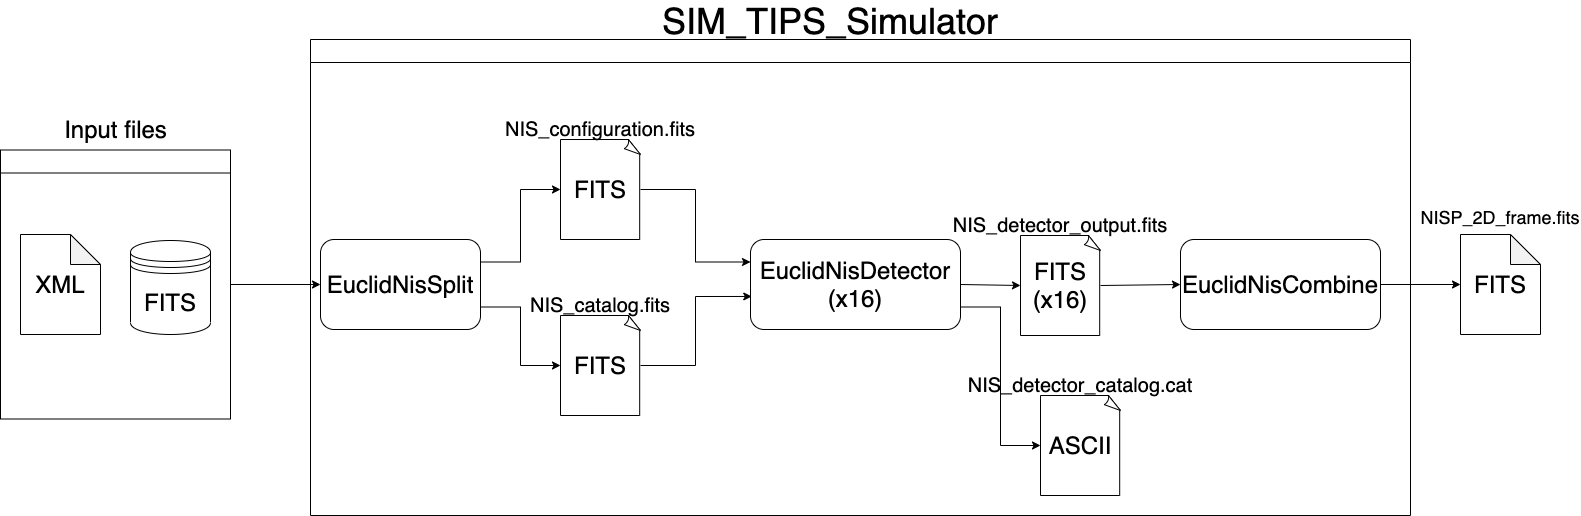
\includegraphics[scale=0.25]{figures/TIPS_workflow.png}
    \caption{Schematic representation of the workflow of TIPS.}
    \label{fig:TIPS_workflow}
\end{figure}



\subsection{Input files}

